\documentclass{article}
\usepackage{graphicx} % Required for inserting images
\usepackage[italian]{babel}
\usepackage{xcolor}
\usepackage{amsmath}
\usepackage{float}
\usepackage{multicol}
\usepackage{changepage}
\usepackage{algorithm}
\usepackage{algpseudocode}
\usepackage[hidelinks]{hyperref}

\title{Progettazione di sistemi digitali}
\author{Leonardo Ganzaroli}
\date{}

\begin{document}

\maketitle

\addcontentsline{toc}{section}{\protect\numberline{}Introduzione}

\tableofcontents

\hypersetup{allcolors=black}

\newpage

\section*{Introduzione}

Questi appunti sono derivanti principalmente dalle slide del corso di \textit{Progettazione di Sistemi Digitali} che ho seguito durante la laurea Triennale di informatica all'università "La Sapienza".

\newpage

\section{Basi numeriche}

I numeri più comunemente utilizzati sono basati sul sistema posizionale, ossia ogni cifra di un numero assume un valore diverso in base alla sua posizione. \newline

\noindent Questo resterà lo standard anche per le altre basi che saranno viste a seguire, l'unica differenza sarà la quantità di simboli usati per rappresentare i numeri.

\subsection{Base Decimale}

La base che viene usata tutti i giorni, usa 0\ldots9.

$$5374_{10} = 5*10^3 + 3*10^2 + 7*10^1 + 4*10^0$$

\subsection{Base Binaria}

Il sistema utlizzato da qualsiasi dispositivo digitale, usa solamente 0 e 1.

$$1101_2 = 1*2^3 + 1*2^2 + 0*2^1 + 1*2^0$$\newline

\noindent Una singola cifra viene definita bit, in un numero binario si individuano 2 bit importanti:

\begin{table}[ht]
    \centering
    \begin{tabular}{ccccc|p{30mm}}
        \textcolor{red}{1} & 1 & 0 & 0 & \textcolor{blue}{1} & \textcolor{red}{Più significativo} \newline \textcolor{blue}{Meno significativo}\\
    \end{tabular}
\end{table}

\subsection{Base Esadecimale}

\vspace{1pt}
Un'altra base che verrà incontrata molto spesso, usa 0\ldots9 e le lettere da A ad F, ha quindi un totale di 16 simboli per rappresentare i numeri.

\vspace{4pt}
\begin{table}[ht]
    \centering
    \begin{tabular}{c|c|c|c|c|c|c|c|c|c|c|c|c|c|c|c|c}
       \textbf{Decimale} & 0 & 1 & 2 & 3 & 4 & 5 & 6 & 7 & 8 & 9 & 10 & 11 & 12 & 13 & 14 & 15\\
       \hline
       \rule{0pt}{3ex}\textbf{Esadecimale} & 0 & 1 & 2 & 3 & 4 & 5 & 6 & 7 & 8 & 9 & A & B & C & D & E & F
    \end{tabular}
    \caption{Corrispondenza tra basi}
    \label{tab:dec_hex_corr}
\end{table}

\newpage

\subsection{Conversione tra basi}

Dato che l'unica differenza tra le basi sta in quanti simboli usano risulta semplice convertire un numero da una base all'altra.

    \subsubsection{Decimale → Binario}

    Esistono 2 metodi:

    \begin{enumerate}
        \item \begin{itemize}
            \item Trovo la potenza di 2 più grande che sia minore del numero
            \item La sottraggo al numero
            \item Ripeto i punti precedenti usando la differenza della sottrazione fino a raggiungere 0
        \end{itemize}

        \vspace{5pt}
        
        \item \begin{itemize}
            \item Divido il numero per 2
            \item Segno il resto della divisione
            \item Ripeto i punti precedenti usando il quoziente della divisione fino a raggiungere 0
        \end{itemize}
    \end{enumerate}

    \vspace{6pt}
    
    \noindent Alcune potenze del 2 per comodità:
    
    \begin{table}[ht]
        \centering
        \begin{tabular}{c|c|c|c|c|c|c|c|c|c|c}
          Potenza & $2^0$ & $2^1$ & $2^2$ & $2^3$ & $2^4$ & $2^5$ & $2^6$ & $2^7$ & $2^8$ & $2^9$\\
             \hline
          \rule{0pt}{3ex}Numero & 1 & 2 & 4 & 8 & 16 & 32 & 64 & 128 & 256 & 512\\
        \end{tabular}
        \caption{Potenze del 2}
        \label{tab:power}
    \end{table}

    \vspace{3pt}

\noindent\rule{\textwidth}{0.5pt}

    \noindent Per meglio capire i metodi converto il numero 23.

    \vspace{5pt}

    \textbf{Metodo 1}:

    \vspace{2pt}

    \begin{itemize}
    \item$23 - 2^4 = 7$
    \item$7 - 2^2 = 3$
    \item$3 - 2^1 = 1$
    \item$1 - 2^0 = 0$
    \end{itemize}

    \vspace{1pt}

    \noindent Se considero adesso un numero binario come una tabella posso comporlo mettendo 1 nelle colonne delle potenze usate + 1 (da dx a sx).
    
    \begin{table}[ht]
        \centering
        \begin{tabular}{c|c|c|c|c}
            pos. 5 & pos. 4 & pos. 3 & pos. 2 & pos. 1\\
            \hline
            \rule{0pt}{3ex}1 & 0 & 1 & 1 & 1\\
            \hline
            \rule{0pt}{3ex}$2^4$ & $2^3$ &$ 2^2$ & $2^1$ & $2^0$
        \end{tabular}
    \end{table}

    \vspace{1pt}

    \noindent Quindi $23_{10} = 10111_2$.

    \newpage

    \textbf{Metodo 2}:
    
    \begin{table}[ht]
        \centering
        \begin{tabular}{c|c|c}
            Dividendo & Quoziente & Resto\\
            \hline
            \rule{0pt}{3ex}23 & 11 & 1\\
            11 & 5 & 1\\
            5 & 2 & 1\\
            2 & 1 & 0\\
            1 & 0 & 1
        \end{tabular}
    \end{table}

Basta adesso leggere dal basso verso l'alto per avere il numero.

\noindent\rule{\textwidth}{0.5pt}

\vspace{4pt}

\subsubsection{Esadecimale → Binario}

Per convertire basta associare ad ogni simbolo esadecimale il rispettivo valore binario:

\begin{table}[ht]
    \centering
    \begin{tabular}{c|c}
        0 & 0000\\
        \hline
        \rule{0pt}{3ex}1 & 0001\\
        \hline
        \rule{0pt}{3ex}2 & 0010\\
        \hline
        \rule{0pt}{3ex}3 & 0011\\
        \hline
        \rule{0pt}{3ex}4 & 0100\\
        \hline
        \rule{0pt}{3ex}5 & 0101\\
        \hline
        \rule{0pt}{3ex}6 & 0110\\
        \hline
        \rule{0pt}{3ex}7 & 0111\\
        \hline
        \rule{0pt}{3ex}8 & 1000\\
        \hline
        \rule{0pt}{3ex}9 & 1001\\
        \hline
        \rule{0pt}{3ex}A & 1010\\
        \hline
        \rule{0pt}{3ex}B & 1011\\
        \hline
        \rule{0pt}{3ex}C & 1100\\
        \hline
        \rule{0pt}{3ex}D & 1101\\
        \hline
        \rule{0pt}{3ex}E & 1110\\
        \hline
        \rule{0pt}{3ex}F & 1111\\
    \end{tabular}
    \caption{Associazione}
    \label{tab:hex_bin}
\end{table}

Per convertire 4AF16 prendo l'equivalente in binario e sostituisco:

$$ 4 = 0100,\
 A = 1010,\ 
 F = 1111,\ 
 1 = 0001,\ 
 6 = 0110$$

Concatenando i risultati ottengo $4AF16_{16} = 01001010111100010110_2$

\newpage

\section{Numeri binari}

Andiamo adesso ad approfondire i numeri binari che saranno la base fondamentale utilizzata da qui in poi.

\subsection{Unità di misura}

Alcune unità utili sono:

\begin{itemize}
    \item Bit = un singolo 0/1
    \item Byte = 8 bit
    \item Nibble = 4 bit = Mezzo byte
    \item Kilobyte = 1024 byte
    \item Megabyte = 1024 kilobyte
    \item \ldots
\end{itemize}

\subsection{Operazioni aritmetiche}

Le operazioni hanno il medesimo funzionamento della loro controparte decimale.

\subsubsection{Somma}

\begin{table}[ht]
    \centering
    \begin{tabular}{|c|c|c|}
        \hline
        + & 0 & 1\\
        \hline
        0 & 0 & 1\\
        \hline
        1 & 1 & 10\\
        \hline
    \end{tabular}
    \caption{Tabella delle somme}
    \label{tab:sum_tab}
\end{table}

\vspace{5pt}

\noindent\rule{\textwidth}{0.5pt}

\noindent Per esempio $91+109=200$:

\[
\begin{array}{c@{}c@{}c@{}c@{}c@{}c@{}c@{}c}
   & _1 & _1 & _1 & _1 & _1 & _1 &   \\
   & 1 & 0 & 1 & 1 & 0 & 1 & 1 \\
+  & 1 & 1 & 0 & 1 & 1 & 0 & 1 \\
\hline
   1 & 1 & 0 & 0 & 1 & 0 & 0 & 0 \\
\end{array}
\]

\noindent\rule{\textwidth}{0.5pt}

\subsubsection{Sottrazione}

La sottrazione si può svolgere con il metodo classico oppure come vedremo tra poco si può ricondurre ad una somma con un numero negativo.

\newpage

\subsubsection{Moltiplicazione}
 
\begin{table}[ht]
    \centering
    \begin{tabular}{|c|c|c|}
        \hline
        $\times $ & 0 & 1\\
        \hline
        0 & 0 & 0\\
        \hline
        1 & 0 & 1\\
        \hline
    \end{tabular}
    \caption{Tabella moltiplicativa}
    \label{tab:mult_tab}
\end{table}

\noindent\rule{\textwidth}{0.5pt}

\noindent Esempio $91 \times 5 = 455$:

\[
\begin{array}{c@{}c@{}c@{}c@{}c@{}c@{}c@{}c@{}c@{}c@{}}
   & & & 1 & 0 & 1 & 1 & 0 & 1 & 1 \\
 * & & & &  &  &  & 1 & 0 & 1 \\
\hline
 + & & & 1 & 0 & 1 & 1 & 0 & 1 & 1 \\
 + & & 0 & 0 & 0 & 0 & 0 & 0 & 0 & \\
 + & 1 & 0 & 1 & 1 & 0 & 1 & 1 & \\
  \hline
  & 1 & 1 & 1 & 0 & 0 & 0 & 1 & 1 & 1
\end{array}
\]

\noindent\rule{\textwidth}{0.5pt}

\subsection{Overflow}

L'overflow è un problema che si presenta quando un'operazione restituisce un risultato con più bit di quanti se ne possono rappresentare, in questo caso i bit "in più" verranno scartati e questo può portare a dei risultati incorretti.

\subsection{Numeri negativi}

Per rappresentare in binario i numeri negativi ho 2 alternative:

\begin{itemize}
    \item \textbf{Sign/Magnitude}

        \vspace{2pt}

        Uso il bit più significativo per indicare il segno del numero.

        \vspace{3pt}
        
        Questo metodo ha 3 problemi:
        \begin{enumerate}
            \item Con $x$ bit posso rappresentare solo $2^{x-1}$ valori invece di $2^x$
            \item Ho 2 rappresentazioni dello 0 → $00,10$
            \item L'addizione non funziona
        \end{enumerate}

    \item \textbf{Complemento a 2}

        \vspace{2pt}

        Il bit più significativo assume il suo effettivo valore, ma se è uguale ad 1 quel valore sarà considerato negativo.

        \vspace{3pt}
            
        Questo metodo risolve i problemi dell'altro, serve però una piccola "trasformazione" per portare un numero in complemento a 2.

\end{itemize}

\subsubsection{Complemento a 2}

Per ottenere un numero in complemento a 2 ci sono 2 passaggi:
\begin{enumerate}
    \item Inverto tutti i bit (Complemento ad 1)

    \item Sommo 1 al numero ottenuto

\end{enumerate}

\vspace{3pt}

\noindent\rule{\textwidth}{0.5pt}

    \noindent Per rappresentare -25:

    \begin{itemize}
        \item $ 25 = 011001 $→$ 100110$
        \item $ 100110 + 1 = 100111$
    \end{itemize}

\noindent Ottengo $100111 = -1*2^5 + 0*2^4 + 0*2^3
+ 1*2^2 +1*2^1 + 1*2^0 = -25$

\noindent\rule{\textwidth}{0.5pt}

\subsection{Numeri razionali}

Anche in questo caso ci sono 2 metodi di rappresentazione.

\subsubsection{Virgola fissa}

Si scelgono due quantità di bit che andranno a rappresentare rispettivamente la parte intera e quella decimale, il "punto" viene inserito implicitamente tra le due parti.\newline

\noindent\rule{\textwidth}{0.5pt}

\noindent Se per esempio si decide di usare 4 bit per entrambe le parti:

\begin{table}[ht]
    \centering
    \begin{tabular}{cccc|cccc}
        0 & 1 & 1 & 0 & 1 & 1 & 0 & 0\\
        \hline
        \rule{0pt}{3ex}$2^3$ & $2^2$ & $2^1$ & $2^0$ & $2^{-1}$ & $2^{-2}$ & $2^{-3}$ & $2^{-4}$\\
    \end{tabular}
    \caption{$6.75$}
    \label{tab:fixpoint_num}
\end{table}

\vspace{-15pt}

\noindent\rule{\textwidth}{0.5pt}

\vspace{-7pt}

\subsubsection{Virgola mobile}

Questo sistema è simile alla notazione scientifica, i numeri vengono trattati quindi nella forma: $$\pm \ \text{Mantissa}\times\text{Base}^{\text{Esponente}}$$

\noindent Solitamente si lavora con stringhe di bit di lunghezza prefissata, le 2 più comuni sono:

\begin{table}[ht]
    \centering
    \begin{tabular}{c|c|c|c|c}
         Precisione & Lunghezza & Segno & Esponente & Mantissa\\
         \hline
         \rule{0pt}{3ex}Singola & 4 byte & 1 bit & 1 byte & 23 bit\\
         \hline
         \rule{0pt}{3ex}Doppia & 5 byte & 1 bit & 11 bit & 52 bit
    \end{tabular}
    \label{tab:floatpoint_num}
\end{table}

\newpage

\noindent Per convertire un numero in questo formato si seguono questi passaggi:
\begin{enumerate}
    \item Trasformare il numero in virgola fissa \textbf{senza segno}
    \item Riscriverlo in notazione scientifica binaria
    \item Riempire i campi
        \begin{itemize}
            \item Ignorare il primo 1 nella mantissa
            \item L'esponente va sommato a 127 (Standard IEEE 754, se Double 1023)
        \end{itemize}
\end{enumerate}

\vspace{5pt}

\noindent\rule{\textwidth}{0.5pt}

\noindent Per esempio ($-11.625$):

\begin{enumerate}
    \item In virgola fissa senza segno = $1011.101$
    \item In notazione = $1.011101\times 2^3$
    \item Riempo i campi
        \begin{itemize}
            \item $\text{Segno} = 1$
            \item $\text{Esponente} = 127+3 = 130 =10000010 $
            \item $\text{Mantissa} = 011101$
        \end{itemize}
    \begin{table}[ht]
        \centering
        \begin{tabular}{|c|c|c|}
            \hline
             \rule{0pt}{1ex}1 & 10000010 & 011101000\ldots \\
             \hline
        \end{tabular}
        \label{tab:example_floatpoint}
    \end{table}
\end{enumerate}

\noindent\rule{\textwidth}{0.5pt}

\vspace{5pt}

\noindent Sono presenti alcuni valori speciali:

\begin{table}[ht]
    \centering
    \begin{tabular}{|c|c|c|c|}
        \hline
        Numero & Segno & Esponente & Mantissa\\
        \hline
        \rule{0pt}{3ex}0 & X & 00000000 & 0000\ldots\\
        \hline
       \rule{0pt}{3ex}$\infty$ & 0 & 11111111 & 0000\ldots\\
        \hline
        \rule{0pt}{3ex}$-\infty$ & 1 & 11111111 & 0000\ldots\\
        \hline
        \rule{0pt}{3ex}NaN & X & 11111111 & Non-zero\\
        \hline
    \end{tabular}
    \caption{Valori speciali}
    \label{tab:floatpoint_special}
\end{table}

\paragraph{Somma}

Per sommare 2 numeri:
\begin{enumerate}
    \item Portarli in notazione
    \item Portarli allo stesso esponente
    \item Sommare le mantisse
    \item Trasformare il risultato
\end{enumerate}

\newpage

\noindent\rule{\textwidth}{0.5pt}

\noindent Esempio:

\begin{table}[ht]
    \centering
    \begin{tabular}{|c|c|c|c|c|}
        \hline
        $N_1$ & 0 & 10000000 & 0100\ldots & $2.5$\\
        \hline
        $N_2$ & 0 & 10000010 & 10100100\ldots & $13.125$\\
        \hline
    \end{tabular}
\end{table}

\noindent Trasformo in notazione e porto allo stesso esponente:

$$N_1=1.01*2^1$$
$$N_2=1.101001*2^3 = 110.1001*2^1$$

\noindent Sommo:

\[
\begin{array}{c@{}c@{}c@{}c@{}c@{}c@{}c@{}c@{}}
   & & & 1. & 0 & 1 \\
 + & 1 & 1 & 0. & 1 & 0 & 0 & 1 \\
\hline
 & 1 & 1 & 1. & 1 & 1 & 0 & 1
\end{array}
\]

\noindent Ritrasformo:

 $$111.1101*2^1=1.111101*2^3$$

\begin{table}[ht]
    \centering
    \begin{tabular}{|c|c|c|c|}
        \hline
        0 & 10000010 & 111101\ldots & $15.625$\\
        \hline
    \end{tabular}
\end{table}

\noindent\rule{\textwidth}{0.5pt}

\section{Logica booleana}

Lavorando con valori binari è essenziale fare una parentesi sulla logica booleana, perché i circuiti logici lavorano con valori binari e il loro funzionamento è espresso tramite equazioni booleane.\newline

\noindent L'algebra di Boole si discosta da quella elementare perché:
\begin{itemize}
    \item Le variabili possono assumere solo 2 valori (di verità):
    \begin{itemize}
        \item Vero
        \item Falso
    \end{itemize}
    \item Le operazioni usate sono quelle logiche:
    \begin{itemize}
        \item AND
        \item OR
        \item NOT
        \item \ldots
    \end{itemize}
\end{itemize}

\newpage

\subsection{Assiomi} 

Alcune formule fondamentali:

\begin{table}[H]
    \begin{adjustwidth}{-3.5cm}{}
    \begin{tabular}{|c|c|c|}
    \hline
        Nome & Teorema & Duale\\
         \hline
        \rule{0pt}{3ex}Identità & $B*1=B$ & $B+0=B$\\
         \hline
        \rule{0pt}{3ex}Elemento nullo & $B*0=0$ & $B+1=1$\\
         \hline
        \rule{0pt}{3ex}Idempotenza & $B*B=B$ & $B+B=B$\\
         \hline
        \rule{0pt}{3ex}Involuzione & \multicolumn{2}{c|}{$B = \bar{\bar{B}}$}\\
         \hline
        \rule{0pt}{3ex}Complemento & $B*\bar{B}=0$ & $B+\bar{B}=1$\\
         \hline
        \rule{0pt}{3ex}Commutatività & $B*C=C*B$ & $B+C=C+B$\\
         \hline
        \rule{0pt}{3ex}Associatività & $B*(C*D) = (B*C)*D$ & $B+(C+D) = (B+C)+D$\\
         \hline
         \rule{0pt}{3ex}Distributività & $B*(C+D) = (B*C)+(B*D)$ & $B+(C*D) = (B+C)*(B+D)$\\
         \hline
        \rule{0pt}{3ex}Assorbimento & $B*(B+C)=B$ & $B+(B*C)=B$\\
         \hline
        \rule{0pt}{3ex}Combinazione & $(B*C)+(B*\bar{C})=B$ & $(B+C)*(B+\bar{C})=B$\\
         \hline
        \rule{0pt}{3ex}Consenso & $(B*C)+(\bar{B}*D)+(C*D)=(B*C)+(\bar{B}*D)$ & $(B+C)*(\bar{B}+D)*(C+D)=(B+C)*(\bar{B}+D)$\\
         \hline
         \rule{0pt}{3ex}De Morgan & $\overline{ABC\ldots} = \bar{A}+\bar{B}+\bar{C}+\bar{\ldots}$ & $\overline{A+B+C\ldots} = \bar{A}\bar{B}\bar{C}\bar{\ldots}$\\
         \hline
    \end{tabular}
    \end{adjustwidth}
    \caption{Assiomi booleani}
    \label{tab:bool_axiom}
\end{table}

\section{Circuiti logici}

Un circuito logico è un insieme di dispositivi digitali interconnessi che può essere visto come una scatola nera, il suo scopo è quello di ricevere un certo numero di input binari e produrre uno o più output binari.\newline

\noindent I valori binari in questione vengono associati fisicamente alla presenza di tensione (1) o meno (0).\newline

\raggedright Essendo trattati come scatole nere vengono utilizzati 4 elementi per descriverli:
\begin{enumerate}
    \item \textbf{Input}
    \item \textbf{Output}
    \item \textbf{Specifiche temporali}
    \item \textbf{Specifiche funzionali}
\end{enumerate}

\newpage

Si possono inoltre distinguere 2 tipi di circuiti:
\begin{enumerate}
    \item \textbf{Combinatori}
        \begin{itemize}
            \item No memoria
            \item L'output dipende solamente dall'input attuale
        \end{itemize}
    \item \textbf{Sequenziali}
            \begin{itemize}
            \item Ha memoria
            \item L'output dipende dall'input attuale e da quelli passati
        \end{itemize}
\end{enumerate}

\subsection{Circuiti combinatori}

Per poter essere definito combinatorio un certo circuito deve necessariamente rispettare alcune regole:
\begin{itemize}
    \item Ogni elemento deve essere combinatorio
    \item Non devono esserci cicli
    \item Ogni nodo è input oppure si connette ad un solo output
\end{itemize}

\subsubsection{Porte logiche}

Una porta logica è uno dei circuiti logici più semplici esistenti, rappresentano la base per creare dei circuiti molto più grandi.\newline

Essendo dei circuiti a loro volta possiamo ignorare gli effettivi componenti interni e descriverne il funzionamento tramite le "tabelle di verità".

\paragraph{Transistor}

I transistor sono dei componenti creati "drogando" il silicio in modo da renderlo conduttivo, sono dei componenti essenziali presenti nella stragrande maggioranza dei dispositivi elettronici.\newline

Hanno 2 principali modalità di funzionamento, una di queste è quella da "switch" (interruttori). Questo li rende degli ottimi candidati per la creazione di porte logiche.\newline

Ne esistono di diversi tipi ma un tipo estremamente adatto è il \textbf{MOSFET}, lo useremo per creare fisicamente le porte.\newline

\newpage

Ne esistono di 2 tipi con funzionamento inverso l'uno dell'altro, la loro combinazione permette di creare le porte:

\begin{figure}[ht]
    \centering
    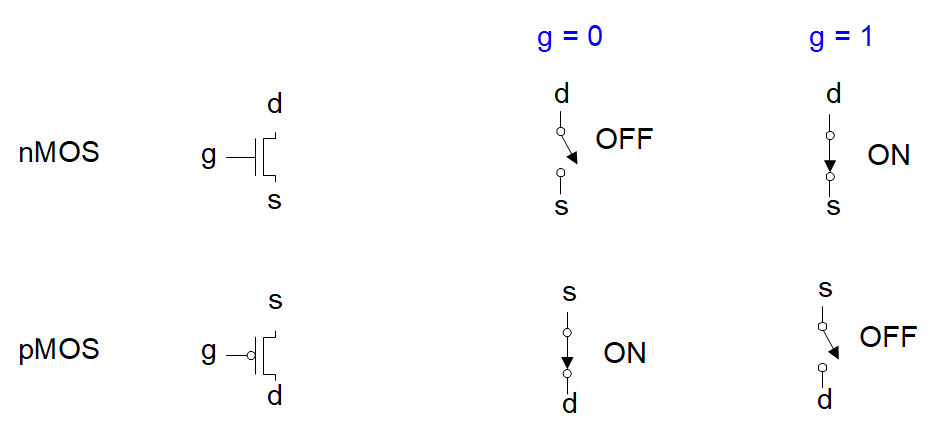
\includegraphics[width=\linewidth]{MOS.png}
    \caption{MOS}
    \label{fig:mos}
\end{figure}

\vspace{10pt}

Lo schema generale per creare delle porte è il seguente:

\begin{figure}[ht]
    \centering
    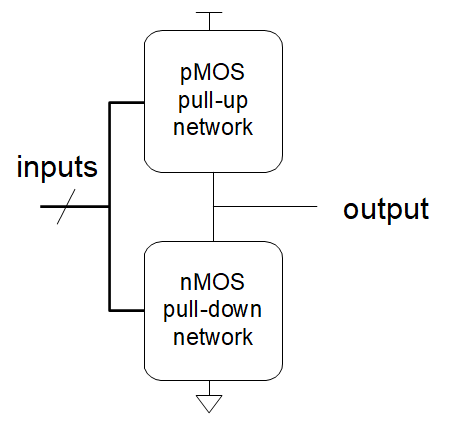
\includegraphics[width=.55\linewidth]{MOS_schema.png}
    \caption{Schema porta logica MOS}
    \label{fig:porta_mos}
\end{figure}

\vspace{5pt}

\textbf{N.B. Le porte create con questo schema sono negate.}

\newpage

\paragraph{Lista delle porte principali}

Le seguenti sono le porte più semplici, con queste si possono creare circuiti più complessi.

\vspace{10pt}

\begin{itemize}

\item \textbf{Buffer}:

\begin{figure}[ht]
    \begin{minipage}[t]{0.49\textwidth}
        \centering
        \begin{figure}[H]
        \centering
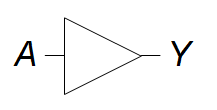
\includegraphics[width=.55\linewidth]{Buffer.png}
        \end{figure}
        \label{fig:buffer}
    \end{minipage}
    \begin{minipage}[t]{0.49\textwidth}
    \centering
        \begin{table}[H]
        \centering
        \begin{tabular}{c|c}
            A & Y\\
            \hline
            0 & 0\\
            \hline
            1 & 1\\
        \end{tabular}
    \label{tab:buffer}
    \end{table}
\end{minipage}
\caption{Buffer}
\end{figure}

\item \textbf{NOT}:

\begin{figure}[ht]
    \begin{minipage}[t]{0.49\textwidth}
        \centering
        \begin{figure}[H]
        \centering
        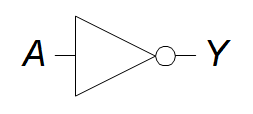
\includegraphics[width=.55\linewidth]{NOT.png}
        \end{figure}
        \label{fig:not}
    \end{minipage}
    \begin{minipage}[t]{0.49\textwidth}
    \centering
        \begin{table}[H]
        \centering
        \begin{tabular}{c|c}
            A & Y\\
            \hline
            0 & 1\\
            \hline
            1 & 0\\
        \end{tabular}
    \label{tab:not}
    \end{table}
\end{minipage}
\caption{NOT}
\end{figure}

\item \textbf{AND}:

\begin{figure}[ht]
    \begin{minipage}[t]{0.49\textwidth}
        \centering
        \begin{figure}[H]
        \centering
        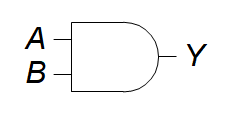
\includegraphics[width=.55\linewidth]{AND.png}
        \end{figure}
        \label{fig:and}
    \end{minipage}
    \begin{minipage}[t]{0.49\textwidth}
    \centering
        \begin{table}[H]
        \centering
        \begin{tabular}{cc|c}
            A & B & Y\\
            \hline
            0 & 0 & 0\\
            \hline
            0 & 1 & 0\\
            \hline
            1 & 0 & 0\\
            \hline
            1 & 1 & 1\\
        \end{tabular}
    \label{tab:and}
    \end{table}
\end{minipage}
\caption{AND}
\end{figure}

\newpage

\item \textbf{OR}:

\begin{figure}[ht]
    \begin{minipage}[t]{0.49\textwidth}
        \centering
        \begin{figure}[H]
        \centering
        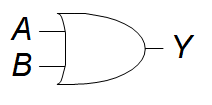
\includegraphics[width=.55\linewidth]{OR.png}
        \end{figure}
        \label{fig:or}
    \end{minipage}
    \begin{minipage}[t]{0.49\textwidth}
    \centering
        \begin{table}[H]
        \centering
        \begin{tabular}{cc|c}
            A & B & Y\\
            \hline
            0 & 0 & 0\\
            \hline
            0 & 1 & 1\\
            \hline
            1 & 0 & 1\\
            \hline
            1 & 1 & 1\\
        \end{tabular}
    \label{tab:or}
    \end{table}
\end{minipage}
\caption{OR}
\end{figure}

\item \textbf{XOR}:

\begin{figure}[ht]
    \begin{minipage}[t]{0.49\textwidth}
        \centering
        \begin{figure}[H]
        \centering
        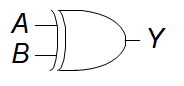
\includegraphics[width=.55\linewidth]{XOR.png}
        \end{figure}
        \label{fig:xor}
    \end{minipage}
    \begin{minipage}[t]{0.49\textwidth}
    \centering
        \begin{table}[H]
        \centering
        \begin{tabular}{cc|c}
            A & B & Y\\
            \hline
            0 & 0 & 0\\
            \hline
            0 & 1 & 1\\
            \hline
            1 & 0 & 1\\
            \hline
            1 & 1 & 0\\
        \end{tabular}
    \label{tab:xor}
    \end{table}
\end{minipage}
\caption{XOR}
\end{figure}

\end{itemize}

\textbf{N.B. Di queste porte esistono anche le versioni con più input.}\newline

Come visto sopra si possono combinare più porte tra loro, per esempio combinando una NOT ed una OR a 3 input:

\begin{figure}[ht]
    \begin{minipage}[t]{0.49\textwidth}
        \centering
        \begin{figure}[H]
        \centering
        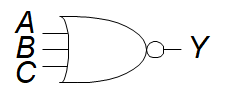
\includegraphics[width=.55\linewidth]{NOR3.png}
        \end{figure}
        \label{fig:nor3}
    \end{minipage}
    \begin{minipage}[t]{0.49\textwidth}
    \centering
        \begin{table}[H]
        \centering
        \begin{tabular}{ccc|c}
            A & B & C & Y\\
            \hline
            0 & 0 & 0 & 1\\
            \hline
            0 & 0 & 1 & 0\\
            \hline
            0 & 1 & 0 & 0\\
            \hline
            0 & 1 & 1 & 0\\
            \hline
            1 & 0 & 0 & 0\\
            \hline
            1 & 0 & 1 & 0\\
            \hline
            1 & 1 & 0 & 0\\
            \hline
            1 & 1 & 1 & 0\\
        \end{tabular}
    \label{tab:nor3}
    \end{table}
\end{minipage}
\caption{NOR3}
\end{figure}

\vspace{5pt}

\textbf{N.B Le porte NAND e NOR sono dette "funzionalmente complete", questo perché possono essere usate per creare tutte le altre porte logiche.}

\vspace{5pt}

\subsubsection{Bubble pushing}

Il bubble pushing è una tecnica che sfrutta il teorema di De Morgan, permette di modificare direttamente il circuito senza passare per le equazioni.\newline

Funzionamento:
\begin{enumerate}
    \item Si parte dall'output
    \item Si spingono le "bolle" verso l'input trasformando la porta
    \item Si tolgono le "bolle" dove possibile
\end{enumerate}

\vspace{4pt}

Partendo da questo schema per esempio:
\begin{figure}[ht]
    \centering
    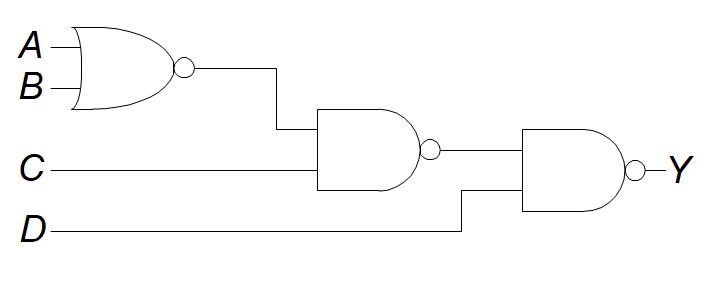
\includegraphics[width=0.52\linewidth]{bpush.png}
    \label{fig:bub_push}
\end{figure}

Svolgo i seguenti passaggi: 

\begin{figure}[ht]
    \centering
    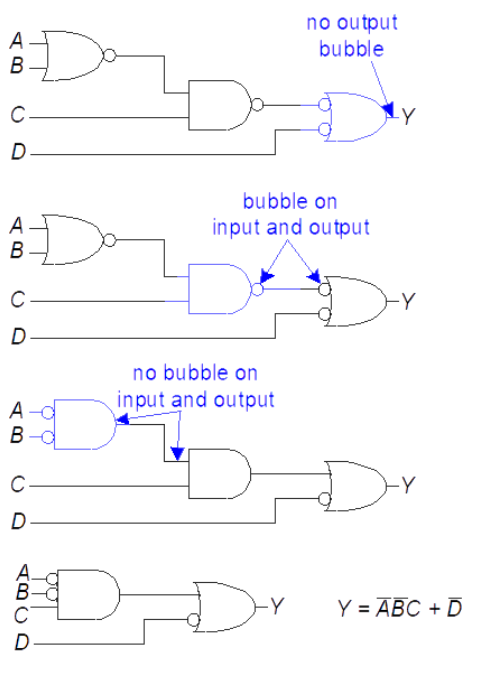
\includegraphics[width=0.52\linewidth]{bpush2.png}
    \caption{Procedimento bubble push}
    \label{fig:bub_push2}
\end{figure}

\subsubsection{Implementazione con MOS}

Come detto prima lo schema usato crea delle porte negate, risulta quindi importante la porta NOT:

\begin{figure}[ht]
    \centering
    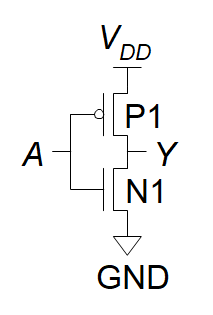
\includegraphics[width=0.25\linewidth]{NOT_MOS.png}
    \caption{NOT MOS}
    \label{fig:not_mos}
\end{figure}

Altre 2 porte sono:

\begin{figure}[ht]
    \centering
    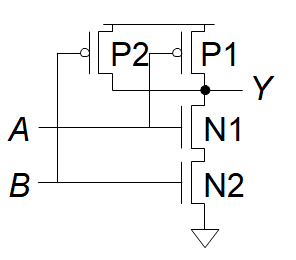
\includegraphics[width=0.31\linewidth]{NAND_MOS.png}
    \caption{NAND MOS}
    \label{fig:nand_mos}
\end{figure}


\begin{figure}[ht]
    \centering
    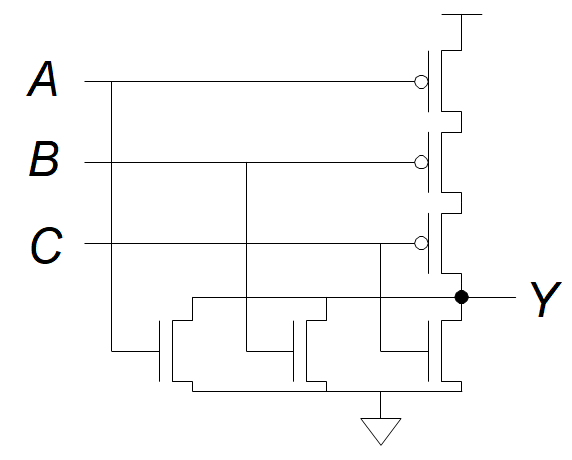
\includegraphics[width=0.31\linewidth]{NOR3_MOS.png}
    \caption{NOR3 MOS}
    \label{fig:nor3_mos}
\end{figure}

In breve:
\begin{itemize}
    \item AND = serie sotto, parallelo sopra
    \item OR = parallelo sotto, serie sopra
\end{itemize}

\subsubsection{Livelli logici}

L'uso di livelli di tensione come input può portare dei problemi dovuti a: 
\begin{itemize}
    \item Rumore termico
    \item Interferenze elettromagnetiche
\end{itemize} 

In caso i valori vengano sballati in modo importante da una di quest'ultime possono esserci dei problemi di falsa lettura, per ovviare al problema vengono stabiliti dei margini per cercare di contrastare il problema e si stabilisce una zona "proibita" tra i 2.

\begin{figure}[ht]
    \centering
    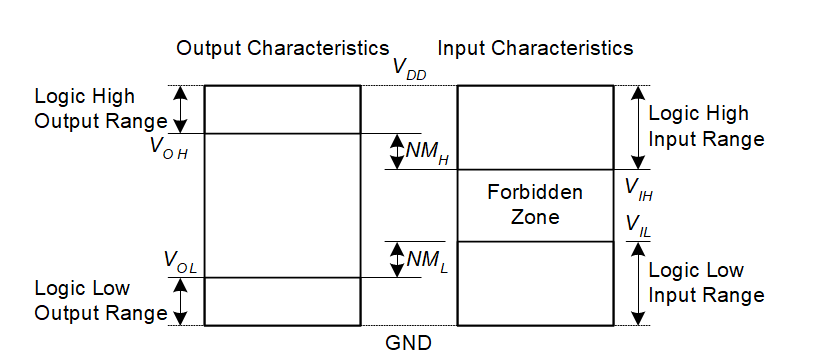
\includegraphics[width=\linewidth]{margini.png}
    \caption{Creazione margini}
    \label{fig:margini}
\end{figure}

\subsubsection{Ritardi}

Un ulteriore problema è quello dei ritardi che si sviluppano nei circuiti, questi sono dovuti a fenomeni fisici come la generazione del calore da parte dei componenti o l'uso di componenti con diverse caratteristiche.\newline

Anche questo fenomeno può portare a false letture (se un singolo cambiamento in input ne comporta diversi in output si parla di \textit{Glitch}), i 2 ritardi più importanti sono:

\begin{itemize}
    \item Ritardo di propagazione
    \item Ritardo di contaminazione
\end{itemize}

Sono rispettivamente il tempo massimo e minimo trascorso dal cambio di input a quello di output, di conseguenza si individuano in un circuito due percorsi:
\begin{itemize}
    \item Critico (o lungo)
    \item Breve
\end{itemize}

\subsubsection{Equazioni booleane}

Il modo in cui si può esprimere l'output di un crcuito partendo dall'input.

\paragraph{Definizioni}

\begin{itemize}
    \item \textbf{Letterale} = Variabile o suo complemento
    \item \textbf{Complemento} = Letterale con barra superiore ($\bar{A}$)
    \item \textbf{Prodotto} = AND = * = Letterali senza spazio tra loro (ABD)
    \item \textbf{Somma} = OR = +
    \item \textbf{Implicante} = Prodotto di letterali
    \item \textbf{Mintermine} = Prodotto che include tutti gli input
    \item \textbf{Maxtermine} = Somma che include tutti gli input
    \item \textbf{Analisi} = Circuito → Equazione
    \item \textbf{Sintesi} = Equazione → Circuito
\end{itemize}

\paragraph{SOP/POS}

2 forme in cui può essere scritta ogni equazione:
\begin{itemize}
    \item \textbf{SOP} (Somma di prodotti) 
        \begin{itemize}
            \item Ogni riga ha un mintermine
            \item Prendo le righe con output 1
            \item Complemento se input è 0
        \end{itemize}
    \item \textbf{POS} (Prodotto di somme)
            \begin{itemize}
            \item Ogni riga ha un maxtermine
            \item Prendo le righe con output 0
            \item Complemento se input è 1
        \end{itemize}
\end{itemize}

\noindent\rule{\textwidth}{0.5pt}

Esempio:
    
    \begin{table}[ht]
        \centering
        \begin{tabular}{cc|c|c|c}
            A & B & Y & Maxt & Mint\\
            \hline
            \rule{0pt}{3ex}0 & 0 & 0 & $A+B$ & $\bar{A}\bar{B}$\\
            0 & 1 & 1 & $A+\bar{B}$ & $\bar{A}B$\\
            1 & 0 & 0 & $\bar{A}+B$ & $A\bar{B}$\\
            1 & 1 & 1 & $\bar{A}+\bar{B}$ & $AB$\\
        \end{tabular}

    \end{table}

$$SOP = \bar{A}B+AB$$
$$POS=(A+B)(\bar{A}+B)$$

\noindent\rule{\textwidth}{0.5pt}

\paragraph{Semplificazione}

Applicando gli assiomi booleani è possibile semplificare equazioni complesse:

\begin{equation}
\nonumber
\begin{split}
    Y = & AB+BC+\bar{B}\bar{D}+A\bar{C}\bar{D}\\ 
    & AB+BC+\bar{B}\bar{D}+A\bar{C}\bar{D}+A\bar{D} \text{ (Consenso)}\\
    & AB+BC+\bar{B}\bar{D}+(A\bar{C}\bar{D}+A\bar{D}) \text{ (Associatività)}\\
    & AB+BC+\bar{B}\bar{D}+A\bar{D} \text{ (Assorbimento)}\\
    & AB+BC+\bar{B}\bar{D} \text{ (Consenso)}
\end{split}
\end{equation}

\subsubsection{Mappe di Karnaugh}

Le mappe di Karnaugh sono un modo grafico per minimizzare le equazioni booleane di massimo 4 variabili, usandole si ottiene una forma SOP (o POS) minima dell'equazione.\newline

\paragraph{X e Z}

Si tratta di 2 valori speciali che possono essere incontrati:
\begin{itemize}
    \item \textbf{X} → Indica un valore ignoto o che viene ignorato
    \item \textbf{Z} → Indica un valore di alta impedenza
\end{itemize}

\vspace{2pt}

La differenza fondamentale tra i 2 è che Z può essere cambiato in presenza di un altro segnale elettrico, come nel caso del buffer tri-state.\newline

\vspace{5pt}

Per usare le mappe correttamente bisogna seguire delle regole:
\begin{itemize}
    \item Ogni 1 va cerchiato almeno una volta
    \item Ogni cerchio deve contenere $2^n$ elementi in ogni direzione
    \item Il cerchio deve essere il più grande possibile
    \item Il cerchio può estendersi oltre i bordi
    \item I valori X si cerchiano solo se sono utili
    \item Ogni casella è un mintermine
\end{itemize}

\newpage

\noindent\rule{\textwidth}{0.5pt}

Esempio:

\begin{figure}[ht]
    \begin{minipage}[t]{0.49\textwidth}
    \centering
        \begin{table}[H]
        \centering
        \begin{tabular}{cccc|c}
            A & B & C & D & Y\\
            \hline
            0 & 0 & 0 & 0 & 1\\
            0 & 0 & 0 & 1 & 0\\
            0 & 0 & 1 & 0 & 1\\
            0 & 0 & 1 & 1 & 1\\
            0 & 1 & 0 & 0 & 0\\
            0 & 1 & 0 & 1 & 1\\
            0 & 1 & 1 & 0 & 1\\
            0 & 1 & 1 & 1 & 1\\
            1 & 0 & 0 & 0 & 1\\
            1 & 0 & 0 & 1 & 1\\
            1 & 0 & 1 & 0 & 1\\
            1 & 0 & 1 & 1 & 0\\
            1 & 1 & 0 & 0 & 0\\
            1 & 1 & 0 & 1 & 0\\
            1 & 1 & 1 & 0 & 0\\
            1 & 1 & 1 & 1 & 0\\

        \end{tabular}
    \label{tab:k1}
    \end{table}
\end{minipage}
    \begin{minipage}[t]{0.49\textwidth}
        \centering
        \begin{figure}[H]
        \centering
        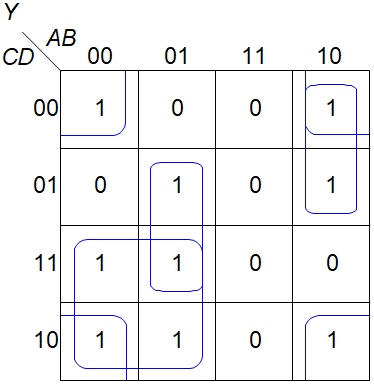
\includegraphics[width=\linewidth]{k1.png}
        \end{figure}
        \label{fig:k1}
    \end{minipage}

    \vspace{10pt}
    Risulta $Y=\bar{A}C+\bar{A}BD+A\bar{B}\bar{C}+\bar{B}\bar{D}$

    \vspace{15pt}

    Se volessi invece la forma POS dovrei:
    \begin{itemize}
        \item Cerchiare gli 0
        \item Considerare ogni casella come maxtermine
        \item Considerare gli 1 come complemento
    \end{itemize}

    \vspace{5pt}

    Otterrei $Y=(\bar{B}+C+D)(\bar{A}+\bar{B})(A+B+C+\bar{D})(\bar{A}+\bar{C}+\bar{D})$
    
\end{figure}

\noindent\rule{\textwidth}{0.5pt}

\newpage

\subsubsection{Altri componenti importanti}

\vspace{5pt}

\begin{itemize}
    \item Multiplexer

    \vspace{5pt}

    Permette di scegliere tramite uno o più segnali quale input collegare all'output:

\begin{figure}[ht]
    \begin{minipage}[t]{0.49\textwidth}
        \centering
        \begin{figure}[H]
        \centering
        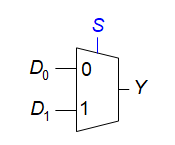
\includegraphics[width=0.6\linewidth]{multiplexer.png}
        \end{figure}
        \label{fig:multiplexer}
    \end{minipage}
    \begin{minipage}[t]{0.49\textwidth}
    \centering
        \begin{table}[H]
        \centering
        \begin{tabular}{c|c}
            S & Y\\
            \hline
            0 & $D_0$\\
            \hline
            1 & $D_1$\\
        \end{tabular}
    \label{tab:multiplexer}
    \end{table}
\end{minipage}
\caption{Multiplexer 2 input}
\end{figure}

\begin{figure}[ht]
    \begin{minipage}[t]{0.49\textwidth}
        \centering
        \begin{figure}[H]
        \centering
        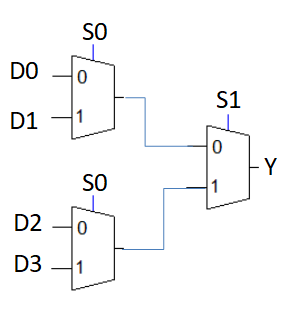
\includegraphics[width=0.8\linewidth]{multiplexer2.png}
        \end{figure}
        \label{fig:multiplexer2}
    \end{minipage}
    \begin{minipage}[t]{0.49\textwidth}
    \centering
        \begin{table}[H]
        \centering
        \begin{tabular}{cc|c}
            $S_1$ & $S_0 $ & Y\\
            \hline
            0 & 0 & $D_0$\\
            \hline
            0 & 1 & $D_1$\\
            \hline
            1 & 0 & $D_2$\\
            \hline
            1 & 1 & $D_3$\\
        \end{tabular}
    \label{tab:multiplexer2}
    \end{table}
\end{minipage}
\caption{Multiplexer 4 input}
\end{figure}

\newpage

\item Decoder

Componente con $x$ input e $2^x$ output, può avere un solo output "attivo" alla volta.

\vspace{5pt}

\begin{figure}[ht]
    \centering
    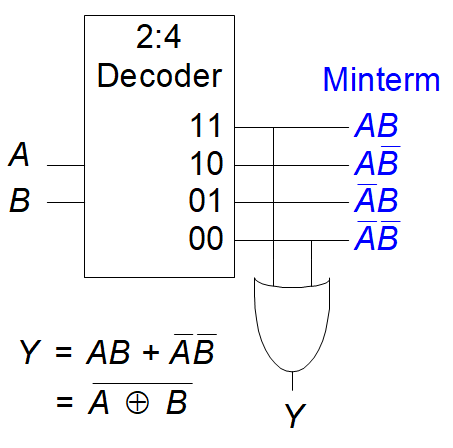
\includegraphics[width=0.55\linewidth]{decoder.png}
    \caption{Decoder con esempio di logica}
    \label{fig:decoder}
\end{figure}
    
\end{itemize}

\subsection{Circuiti sequenziali}

A differenza di quelli combinatori sono presenti dei componenti che permettono di mantenere informazioni riguardo lo stato precedente del sistema.

\subsubsection{Definizioni}

\begin{itemize}
    \item \textbf{Stato} = Tutte le informazioni su un circuito necessarie per spiegare il suo comportamento futuro
    \item \textbf{Latch/Flip-flop} = Elementi che mantengono un bit di stato
    \item \textbf{Circuiti sequenziali sincron}i = Logica combinatoria + banco di flip-flop
\end{itemize}

\newpage

\subsubsection{Elementi di stato}

Gli elementi di stato hanno il compito di conservare lo stato del circuito per influenzarlo nel futuro, i componenti di questo tipo sono:

\begin{itemize}
    \item \textbf{Circuito bistabile}

    Elemento base usato per costruirne altri, ha 2 output, no input e 2 possibili forme:

    \begin{figure}[ht]
        \centering
        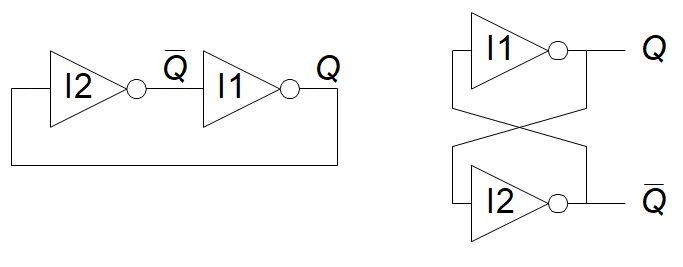
\includegraphics[width=0.8\linewidth]{bistable.png}
        \caption{Circuito bistabile}
        \label{fig:bistable}
    \end{figure}

    Mantiene l'output costante indipendentemente dalla forma e dal fatto che Q sia 1 o 0.

    \vspace{5pt}

    \item \textbf{Latch SR}

    \begin{figure}[ht]
        \begin{minipage}[t]{0.49\textwidth}
            \centering
            \begin{figure}[H]
            \centering
            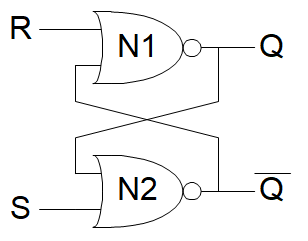
\includegraphics[width=.8\linewidth]{LatchSR.png}
            \end{figure}
            \label{fig:latch_sr}
        \end{minipage}
        \begin{minipage}[t]{0.49\textwidth}
        \centering
            \begin{table}[H]
            \centering
            \begin{tabular}{cc|c|c}
                S & R & Q & $\bar{Q}$\\
                \hline
                \rule{0pt}{3ex}0 & 0 & $Q_{prev}$ & $\bar{Q}_{prev}$\\
                0 & 1 & 0 & 1\\
                1 & 0 & 1 & 0\\
                1 & 1 & \textcolor{red}{0} & \textcolor{red}{0}
            \end{tabular}
        \label{tab:latch_sr}
        \end{table}
    \end{minipage}
    \caption{Latch SR}
    \end{figure}
    
    $S = SET,\  R = RESET$, mantiene lo stato precedente se entrambi sono 0, ha uno stato illegale.

    \newpage

    \item \textbf{Latch D}

        \begin{figure}[ht]
        \begin{minipage}[t]{0.49\textwidth}
            \centering
            \begin{figure}[H]
            \centering
            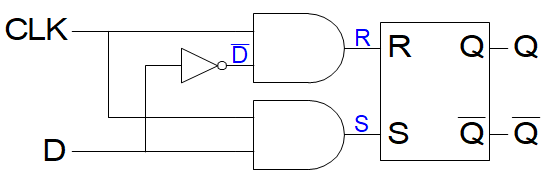
\includegraphics[width=1.1\linewidth]{LatchD.png}
            \end{figure}
            \label{fig:latch_d}
        \end{minipage}
        \begin{minipage}[t]{0.49\textwidth}
        \centering
            \begin{table}[H]
            \centering
            \begin{tabular}{cc|c|c}
                CLK & D & Q & $\bar{Q}$\\
                \hline
                \rule{0pt}{3ex}0 & X & $Q_{prev}$ & $\bar{Q}_{prev}$\\
                1 & 0 & 0 & 1\\
                1 & 1 & 1 & 0
                
            \end{tabular}
        \label{tab:latch_d}
        \end{table}
    \end{minipage}
    \caption{Latch D}
    \end{figure}

    $D = DATA,\  CLK = CLOCK$, mantiene lo stato precedente quando CLK è 0 ed evita lo stato invalido del Latch SR.

    \vspace{5pt}

    \item \textbf{Flip-flop D}

    \begin{figure}[ht]
        \centering
        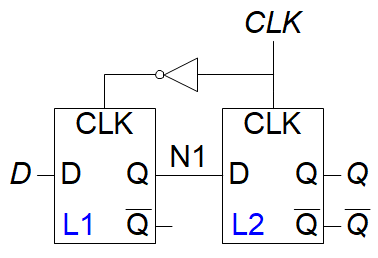
\includegraphics[width=0.65\linewidth]{ffD.png}
        \caption{Flip-flop D}
        \label{fig:ff_D}
    \end{figure}

    $Q = D$ quando il clock sale da 0 a 1, quel valore viene mantenuto fino alla prossima salita del clock.

    \newpage

    \item \textbf{Flip-flop E} (multiplexer + Flip-flop D)

    \begin{figure}[ht]
        \centering
        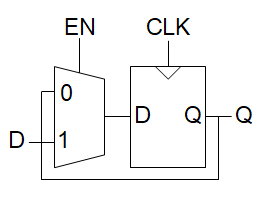
\includegraphics[width=0.5\linewidth]{ffE.png}
        \caption{Flip-flop E}
        \label{fig:ff_E}
    \end{figure}

    Se $EN = 0$ allora mantiene lo stato precedente, altrimenti funziona normalmente.

    \vspace{5pt}

    \item \textbf{Flip-flop R} (AND + Flip-flop D)

    \begin{figure}[ht]
        \centering
        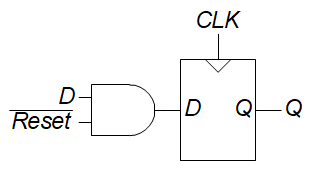
\includegraphics[width=0.6\linewidth]{ffR.png}
        \caption{Flip-flop R}
        \label{fig:ff_R}
    \end{figure}

    Se $RESET = 1$ allora $Q=0$, altrimenti funziona normalmente, il cambio può essere sincrono (aspetta salita clock) o asincrono (istantaneo).

    \newpage

    \item \textbf{Flip-flop S }

    \begin{figure}[ht]
        \centering
        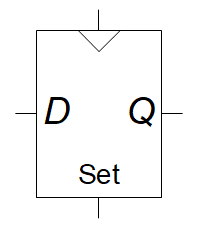
\includegraphics[width=0.3\linewidth]{ffS.png}
        \caption{Flip-flop E}
        \label{fig:ff_S}
    \end{figure}

    Se $SET = 1$ allora $Q=1$, altrimenti funziona normalmente.
    
\end{itemize}

\subsubsection{Circuiti sincroni}

La caratteristica principale di questi circuiti è la loro sincronizzazione con un clock, quindi il loro stato cambierà ad ogni salita del clock.\newline

Devono inoltre rispettare delle regole:
\begin{itemize}
    \item Ogni elemento è un circuito combinatorio o un registro
    \item Tutti i registri usano lo stesso clock 
    \item È presente almeno un registro
    \item Ogni ciclo contiene almeno un registro
\end{itemize}

\vspace{5pt}

I due tipi più comuni sono le FSM e le pipeline.

\newpage

\subsubsection{FSM}

Una macchina a stati finiti è composta da 3 elementi:
\begin{enumerate}
    \item \textbf{Next state logic} → Calcola il valore dello stato successivo
    \item \textbf{Registri} → Conservano lo stato corrente
    \item \textbf{Output Logic} → Si occupa degli output
            
\end{enumerate}

\vspace{5pt}

Ce ne sono 2 tipi:
\begin{itemize}
    \item \textbf{Moore} = output dipendenti solo dallo stato attuale
    \item \textbf{Mealy} = output dipendenti dallo stato attuale e dagli input
\end{itemize}

\begin{figure}[ht]
    \centering
    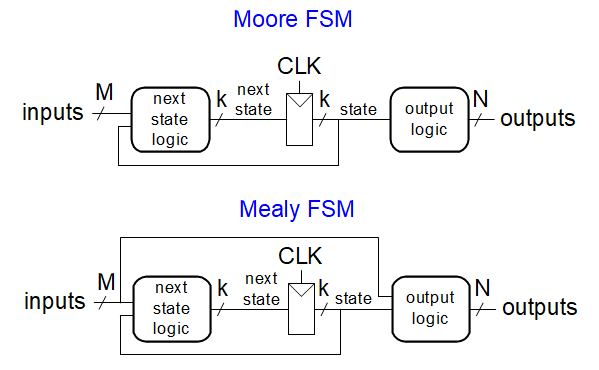
\includegraphics[width=\linewidth]{fsm.png}
    \caption{Schema FSM}
    \label{fig:fsm}
\end{figure}

\paragraph{Diagramma delle transizioni}

Il diagramma delle transizioni si usa per rappresentare graficamente gli stati di una FSM e le transizioni tra di essi.

\begin{itemize}
    \item \textbf{Stati} = Cerchi
    \item \textbf{Transizioni} = Archi
\end{itemize}

\newpage

\noindent\rule{\textwidth}{0.5pt}

Esempio semaforo:

    \begin{figure}[ht]
    \begin{minipage}[t]{0.49\textwidth}
        \centering
        \begin{figure}[H]
        \centering
        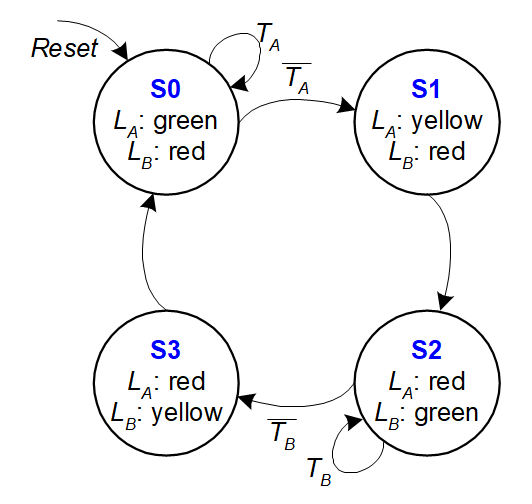
\includegraphics[width=\linewidth]{semaforo.png}
        \end{figure}
        \label{fig:semaforo_fsm}
    \end{minipage}
    \begin{minipage}[t]{0.49\textwidth}
    \centering
    \begin{figure}[H]
    \centering
    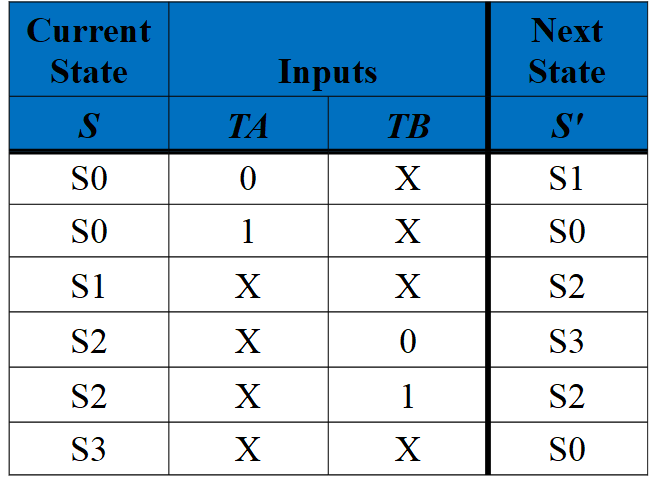
\includegraphics[width=\linewidth]{semaforo_tab.png}
    \end{figure}
    \label{fig:semaforo_tab}
    \end{minipage}
    \caption{Semaforo FSM}
    \end{figure}

Lavorando con i registri bisogna associare ad ogni stato una certa stringa binaria, ci sono 2 alternative:

\vspace{2pt}

\begin{itemize}
    \item Codifica semplice

    \begin{table}[ht]
        \centering
        \begin{tabular}{c|cc}
            Stato & \multicolumn{2}{c}{Stringa} \\
             \hline
             $S_0$ & 0 & 0\\
             $S_1$ & 0 & 1\\
             $S_2$ & 1 & 0\\
             $S_3$ & 1 & 1
        \end{tabular}
        \caption{Cod. semplice}
        \label{tab:cod1}
    \end{table}
    
    \item Codifica One-hot

    \begin{table}[ht]
        \centering
        \begin{tabular}{c|cccc}
            Stato & \multicolumn{4}{c}{Stringa} \\
             \hline
             $S_0$ & 0 & 0 & 0 & 1\\
             $S_1$ & 0 & 0 & 1 & 0\\
             $S_2$ & 0 & 1 & 0 & 0\\
             $S_3$ & 1 & 0 & 0 & 0
        \end{tabular}
        \caption{Cod. 1-hot}
        \label{tab:cod2}
    \end{table}
    
\end{itemize}

\newpage

Usando la prima ottengo:

    \begin{figure}[ht]
    \begin{minipage}[t]{0.49\textwidth}
        \centering
        \begin{figure}[H]
        \centering
        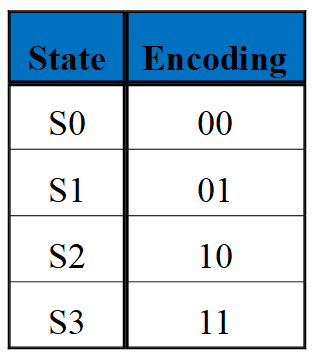
\includegraphics[width=.55\linewidth]{semaforo_cod.png}
        \end{figure}
        \label{fig:semaforo_cod}
    \end{minipage}
    \begin{minipage}[t]{0.49\textwidth}
    \centering
    \begin{figure}[H]
    \centering
    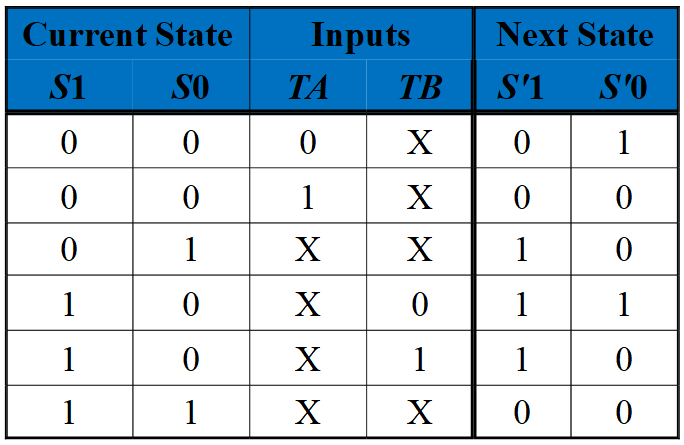
\includegraphics[width=\linewidth]{semaforo_trans.png}
    \end{figure}
    \label{fig:semaforo_trans}
    \end{minipage}
    \caption{Transizioni semaforo}
    \end{figure}

Posso adesso ricavare i valori dei prossimi stati:
\begin{itemize}
    \item $S_1'=S_1\oplus S_0$
    \item $S_0'=\bar{S_1}\bar{S_0}Ta+\bar{S_1}\bar{S_0}T_b$
\end{itemize}

\vspace{5pt}

Faccio la stessa cosa per l'output:

    \begin{figure}[ht]
    \begin{minipage}[t]{0.49\textwidth}
        \centering
        \begin{figure}[H]
        \centering
        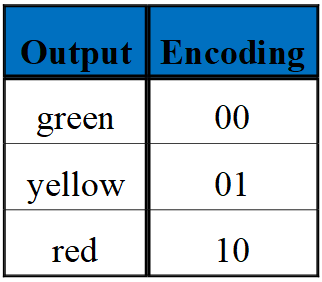
\includegraphics[width=.55\linewidth]{semaforo_cod_out.png}
        \end{figure}
        \label{fig:semaforo_cod_out}
    \end{minipage}
    \begin{minipage}[t]{0.49\textwidth}
    \centering
    \begin{figure}[H]
    \centering
    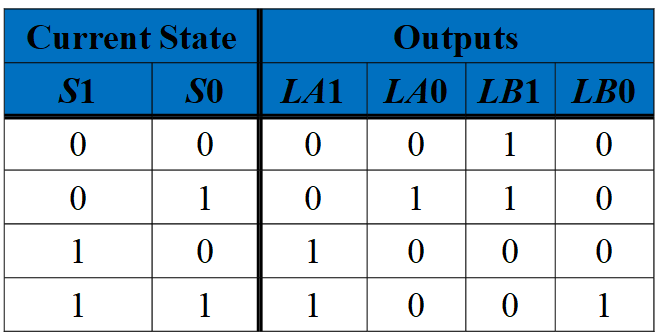
\includegraphics[width=\linewidth]{semaforo_out.png}
    \end{figure}
    \label{fig:semaforo_out}
    \end{minipage}
    \caption{Output semaforo}
    \end{figure}

Ed avrò:
\begin{itemize}
    \item $L_{a1} = S_1$
    \item $L_{a0} = \bar{S_1}S_0$
    \item $L_{b1} = \bar{S_1}$
    \item $L_{b0} = S_1S_0$
\end{itemize}

\newpage

Posso quindi creare lo schema completo:

\begin{figure}[ht]
    \centering
    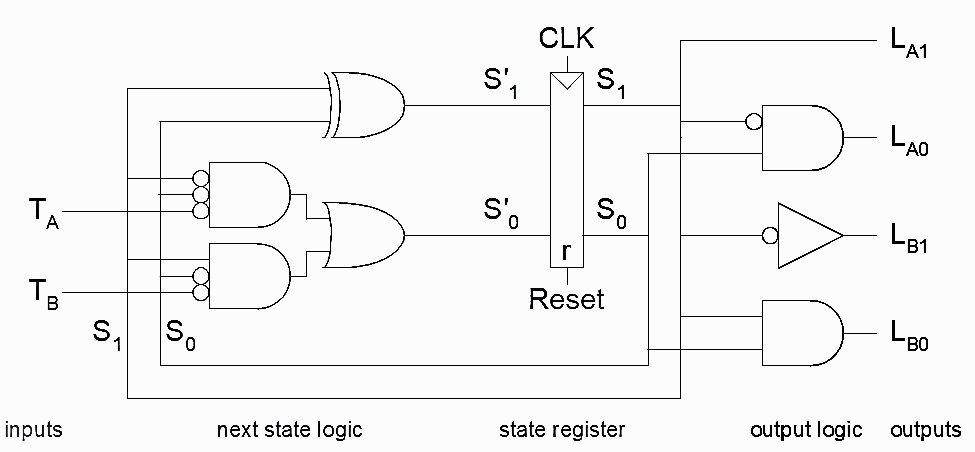
\includegraphics[width=\linewidth]{semaforo_schema.png}
    \caption{Schema semaforo}
    \label{fig:semaforo_schema}
\end{figure}

\noindent\rule{\textwidth}{0.5pt}

\vspace{10pt}

\paragraph{Mealy e Moore}

La differenza tra i 2 tipi sta nella gestione dell'output, uno associa gli output agli stati, l'altro alle transizioni.

\noindent\rule{\textwidth}{0.5pt}

Esempio:

\vspace{3pt}

\begin{figure}[ht]
    \centering
    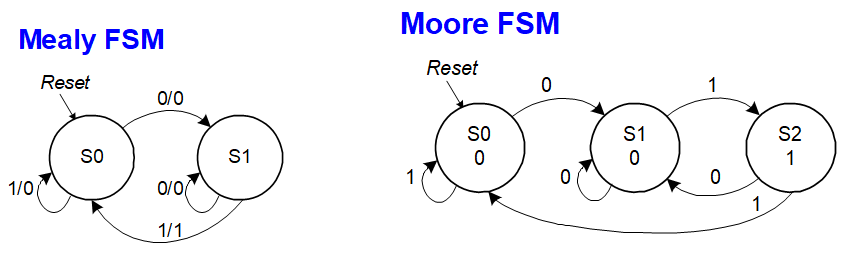
\includegraphics[width=\linewidth]{mm_fsm.png}
    \caption{Differenze}
    \label{fig:fsm_mm}
\end{figure}

Nell'automa di Mealy sugli archi sono indicati gli input/output.

\newpage

La differenza risulta ancora più evidente controllando le tabelle:

    \begin{figure}[ht]
    \begin{minipage}[t]{0.49\textwidth}
        \centering
        \begin{figure}[H]
        \centering
        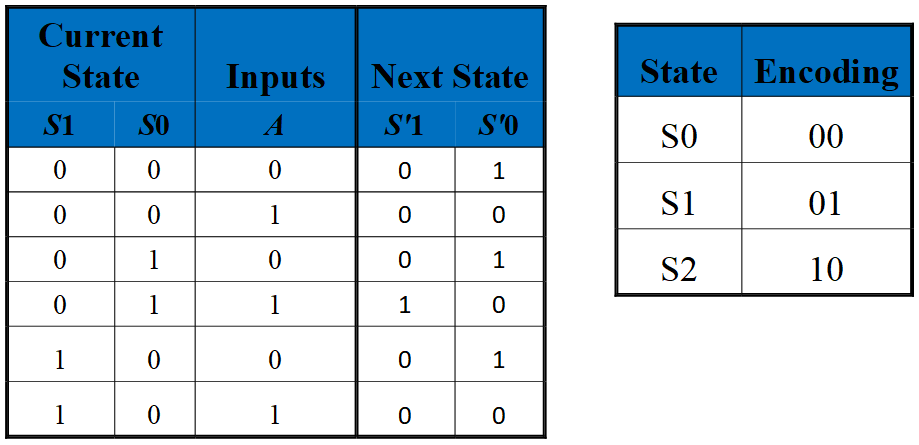
\includegraphics[width=1.1\linewidth]{moore_fsm.png}
        \end{figure}
        \label{fig:moore1}
    \end{minipage}
    \begin{minipage}[t]{0.49\textwidth}
    \centering
    \begin{figure}[H]
    \centering
    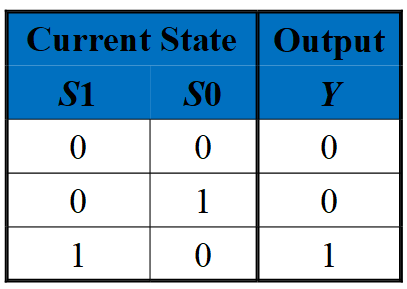
\includegraphics[width=.6\linewidth]{moore_fsm2.png}
    \end{figure}
    \label{fig:moore2}
    \end{minipage}
    \caption{Moore}
    \end{figure}

\begin{figure}[ht]
    \centering
    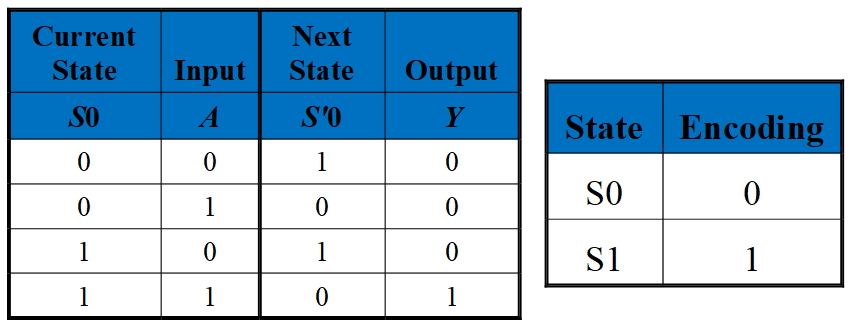
\includegraphics[width=.7\linewidth]{mealy_fsm.png}
    \caption{Mealy}
    \label{fig:mealy}
\end{figure}

\noindent\rule{\textwidth}{0.5pt}

\subparagraph{Intercambiabilità}

Si può passare tranquillamente tra i due tipi di automi seguendo alcuni passaggi:\newline

\textbf{Moore → Mealy}

\vspace{5pt}

Basta spostare l'output dallo stato agli archi entranti in quello stato.\newline

\textbf{Mealy → Moore}

\begin{itemize}
    \item Fare l'opposto del paragrafo predecente
    \item Se ci sono output diversi entranti in un solo stato creare un nuovo stato per ogni output diverso
    \item In caso di nuovi stati aggiungere transizioni per mantenere la logica di funzionamento
\end{itemize}

\newpage

\paragraph{Creazione FSM}

Progettazione:
\begin{enumerate}
    \item Identifica input e output
    \item Disegna il diagramma delle transizioni
    \item Crea la tabella dell transizioni
    \item Codifica gli stati
    \item Crea le equazioni
    \item Crea lo schema
\end{enumerate}

Processo inverso:
\begin{enumerate}
    \item Esamina il circuito
    \item Ricava le equazioni
    \item Crea le tabelle
    \item Se possibile semplifica le tabelle
    \item Assegna ad ogni combinazione valida uno stato
    \item Riscrivi la tabella
    \item Crea il diagramma delle transizioni
\end{enumerate}

\subsubsection{Timing}

Dato il funzionamento dei flip-flop risulta importante che il segnale in ingresso resti stabile durante la salita del clock, in particolare non deve cambiare valore già prima della salita. (Tempo di setup)\newline

Il discorso è simile riguardo l'output, infatti anch'esso dopo la salita potrebbe rimanere instabile per un certo periodo di tempo. (Tempo di hold)\newline

Un ulteriore discorso va fatto riguardo la presenza di registri multipli, funzionando con lo stesso clock ma essendo collegati tramite un circuito servono delle garanzie sulla stabilità nel tempo.\newline

In particolare l'input di $R_2$:
\begin{itemize}
    \item Deve essere stabile per almeno il tempo di setup di $R_2$ prima della salita
    \item Deve essere stabile almeno per il tempo di hold dopo la salita
\end{itemize}

Un ultimo elemento da considerare è il possibile sfasamento del clock tra i vari componenti, infatti ad ognuno potrebbe arrivare in istanti diversi per varie ragioni e creare dei problemi.

\subsection{Parallelismo}

Esistono 2 tipi di parallelismo:
\begin{itemize}
    \item \textbf{Spaziale}

        \quad Dispositivi hardware multipli che svolgono più compiti
        
    \item \textbf{Temporale}
    
        \quad Un certo compito viene diviso in più fasi 
        
\end{itemize}

\vspace{3pt}

Alcune definizioni importanti:
\begin{itemize}
    \item \textbf{Token} = Gruppo di input processati per produrre gruppi di output
    \item \textbf{Latenza} = Tempo impiegato da un token per passare dall'inizio alla fine del circuito
    \item \textbf{Throughput} = Numeri di token processati per unità di tempo
\end{itemize}

\section{Blocchi costruttivi digitali}

Per blocchi costruttivi digitali si intendono tutti gli elementi digitali semplici con funzioni ed interfacce ben strutturate, che possono essere usati come base per sistemi più grandi.\newline

I blocchi in questione sono:
\begin{itemize}
    \item \textbf{Porte logiche}
    \item \textbf{Multiplexer}
    \item \textbf{Decoder}
    \item \textbf{Registri}
    \item \textbf{Contatori}
    \item \textbf{Circuiti aritmetici}
    \item \textbf{Array di memoria}
    \item \textbf{Array logici}
\end{itemize}

\newpage

\subsection{Blocchi aritmetici}

\subsubsection{Sommatori}

Ci sono 2 tipi di sommatori:
\begin{itemize}
    \item \textbf{Half-adder}

        \qquad Esegue la somma degli input ricevuti
    
    \item \textbf{Full-adder}

        \qquad Come sopra ma ha in aggiunta l'input del riporto
    
\end{itemize}

    \begin{figure}[ht]
        \centering
        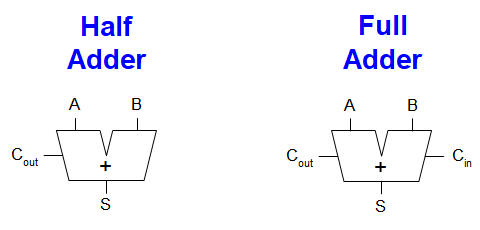
\includegraphics[width=0.8\linewidth]{adder.png}
        \caption{Sommatori}
        \label{fig:adder}
    \end{figure}

\begin{figure}[ht]
    \begin{minipage}[t]{0.49\textwidth}
        \centering
        \begin{table}[H]
        \centering
        \begin{tabular}{cc|cc}
            A & B & $C_{out}$ & S\\
            \hline
            0 & 0 & 0 & 0\\
            0 & 1 & 0 & 1\\
            1 & 0 & 0 & 1\\
            1 & 1 & 1 & 0
        \end{tabular}
    \label{tab:half_add}
    \end{table}
    $S=A\oplus B$,
    $C_{out}=AB$
    \end{minipage}
    \begin{minipage}[t]{0.49\textwidth}
    \centering
        \begin{table}[H]
        \centering
        \begin{tabular}{ccc|cc}
            $C_{in}$ & A & B & $C_{out}$ & S\\
            \hline
            0 & 0 & 0 & 0 & 0\\
            0 & 0 & 1 & 0 & 1\\
            0 & 1 & 0 & 0 & 1\\
            0 & 1 & 1 & 1 & 0\\
            1 & 0 & 0 & 0 & 1\\
            1 & 0 & 1 & 1 & 0\\
            1 & 1 & 0 & 1 & 0\\
            1 & 1 & 1 & 1 & 1
        \end{tabular}
    \label{tab:full_add}
    \end{table}
    $S=A\oplus B \oplus C$,
    $C_{out}=AB+AC_{in}+BC_{in}$
\end{minipage}
\end{figure}

In caso di sommatori a più bit ci sono 3 modi per passare i riporti:
\begin{enumerate}
    \item Ripple-carry
    \item Carry-lookahead
    \item Prefix
\end{enumerate}

\newpage

\paragraph{Ripple-carry}

Il modo più semplice ma anche il più lento, semplicemente vengono messi in catena i sommatori.

\begin{figure}[ht]
    \centering
    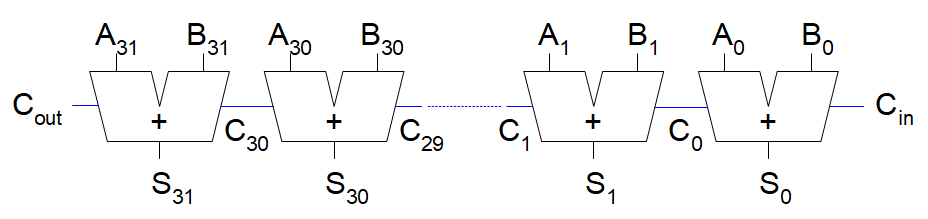
\includegraphics[width=\linewidth]{adder_chain.png}
    \caption{Catena di adder}
    \label{fig:adder_chain}
\end{figure}

\paragraph{Carry-lookahead}

Un certo sommatore in una catena può generare un riporto oppure propagare quello in input, sottoforma di equazioni diventa:
\begin{itemize}
    \item \textbf{Genera} $= AB$
    \item \textbf{Propaga} $= A+B$
    \item \textbf{Riporto in uscita} $= AB+(A+B)C_{in}$
\end{itemize}

\vspace{2pt}

A questo punto posso dividere la catena in blocchi di lunghezza uguale ed usare questo metodo per passare il riporto dai blocchi precedenti a quelli successivi, in questo modo si va a ridurre il tempo di attesa.\newline

La formula generica per un blocco diventa: \begin{align*}
    P_{i:j} &= P_i * P_{i-1} * P_{i-2} \ldots * P_j\\
    G_{i:j} &= G_i + P_i(G_{i-1}+P_{i-1}(G_{i-2}\ldots*G_j))\ldots\\
    C_i &= G_{i:j}+P_{i:j}*C_{j-1}  
\end{align*}

\newpage

\begin{figure}[ht]
    \centering
    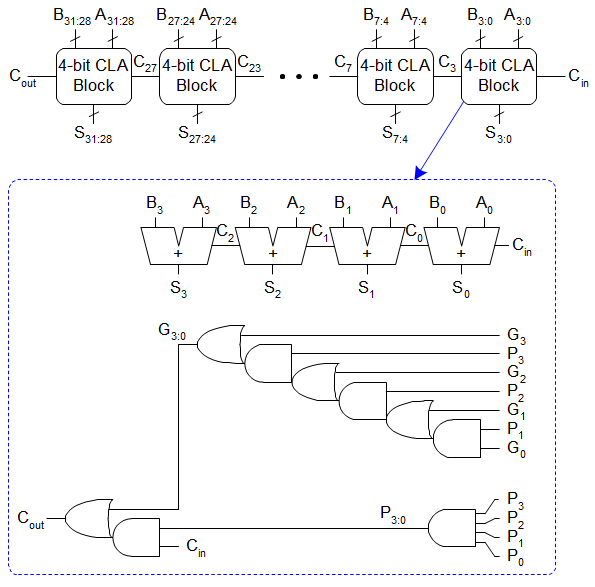
\includegraphics[width=\linewidth]{adder_carry.png}
    \caption{Schema Carry-lookahead}
    \label{fig:carry-lookahead}
\end{figure}

\newpage

\subsubsection{Sottrattori}

Basta sommare B in complemento a 1 (negandolo) e aggiungere 1 tramite $C_{in}$:

\begin{figure}[ht]
    \centering
    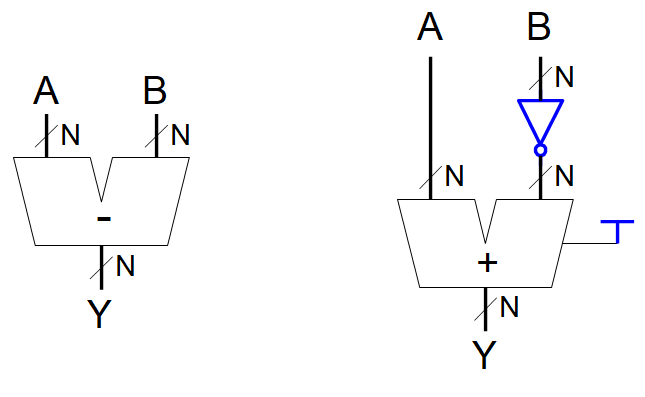
\includegraphics[width=0.7\linewidth]{subtracter.png}
    \caption{Sottrattore}
    \label{fig:enter-label}
\end{figure}

\subsubsection{Comparatori}

Per controllare se due stringhe sono uguali basta usare una porta XNOR usando come input l'iesimo bit di entrambe le stringhe e poi fare un AND di tutte le porte XNOR.

\begin{figure}[ht]
    \centering
    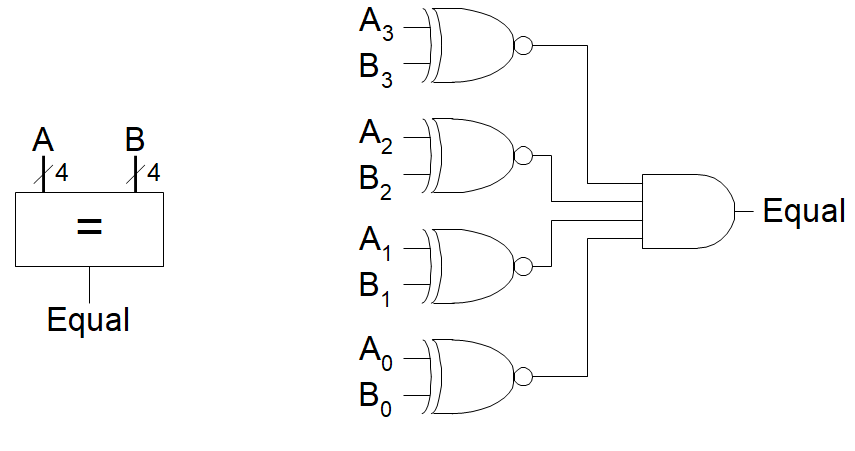
\includegraphics[width=\linewidth]{comp.png}
    \caption{Comparatore eguaglianza}
    \label{fig:comp}
\end{figure}

\subsubsection{Shifter}

Traslano la stringa a destra o a sinistra:
\begin{itemize}
    \item \textbf{Logico}
    
    Sposta gli elementi della stringa di un certo numero di posizioni a destra o sinistra, inserisce 0 negli spazi rimasti vuoti.

    $11011 >> 2 = \textbf{00}110$, $11011<<2=011\textbf{00}$

\begin{figure}[ht]
    \centering
    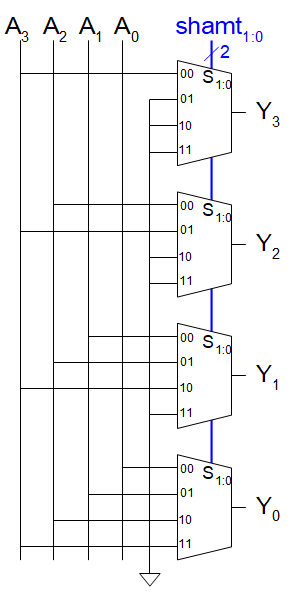
\includegraphics[width=0.45\linewidth]{shifter.png}
    \caption{Shifter DX nibble}
    \label{fig:shifter}
\end{figure}
        
    \item \textbf{Aritmetico}
    
    Uguale al logico ma quello a dx riempe con il MSB.
    
    \item \textbf{Rotatore}
    
    Ruota un certo numero di bit all'altra estremità della stringa.

    $11011\ ROL\ 2 = 110\textbf{11}$, $11011\ ROR\ 2=\textbf{11}110$
    
\end{itemize}

\newpage

\subsection{Memorie}

Matrici di bit usate per contenere grandi quantità di dati, hanno:
\begin{itemize}
    \item $2^x$ righe con $x$ input d'indirizzo
    \item Colonne pari agli input/output dati
\end{itemize}

\begin{figure}[ht]
    \centering
    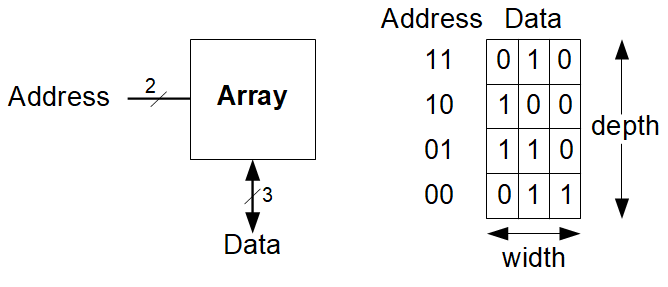
\includegraphics[width=0.65\linewidth]{mem_array.png}
    \caption{Array $2\times 3$}
    \label{fig:mem_array}
\end{figure}

Per leggere una singola cella bisogna dare in input l'indirizzo della stringa e poi leggere l'output dati giusto.

\begin{figure}[ht]
    \begin{minipage}[t]{0.49\textwidth}
    \begin{figure}[H]
        \centering
        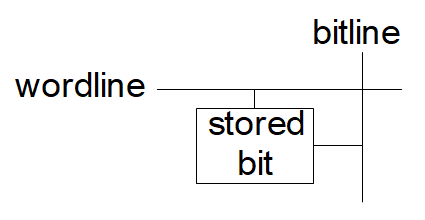
\includegraphics[width=0.6\linewidth]{mem_cell.png}
        \label{fig:mem_cell}
    \end{figure}
    \end{minipage}
    \begin{minipage}[t]{0.49\textwidth}
    \centering
        \begin{table}[H]
        \centering
        \begin{tabular}{cc|c}
            wordline & stored bit & bitline\\
            \hline
            0 & X & Z\\
            1 & 0 & 0\\
            1 & 1 & 1\\
        \end{tabular}
    \label{tab:mem_cell}
    \end{table}
\end{minipage}
\caption{Singola cella di memoria}
\end{figure}

\paragraph{Tipi di memorie}

\begin{itemize}

    \item \textbf{RAM} (Random access memory)
        \begin{itemize}
            \item Volatile = Perde i dati senza corrente
            \item Lettura/scrittura veloce
        \end{itemize}

        Ci sono 2 tipi di RAM:
        \begin{itemize}
            \item \textbf{DRAM} (Dinamica)
            \item \textbf{SRAM} (Statica)
        \end{itemize}

        La differenza sta nel modo di immagazzinare i dati.
    
    \item \textbf{ROM} (Read only memory)
        \begin{itemize}
            \item Non volatile = Mantiene i dati senza corrente
            \item Lettura veloce
            \item Solitamente solo lettura
        \end{itemize}
\end{itemize}

\paragraph{Logica}

Data la struttura ed il fuzionamento delle memorie si può sfruttare un decoder per la gestione degli indirizzi e rappresentare la matrice tramite la \textbf{Dot Notation}, in questo modo si possono utilizzare per compiere logica tramite gli output (visti come equazioni).

\begin{figure}[ht]
    \begin{minipage}[t]{0.49\textwidth}
    \begin{figure}[H]
        \centering
        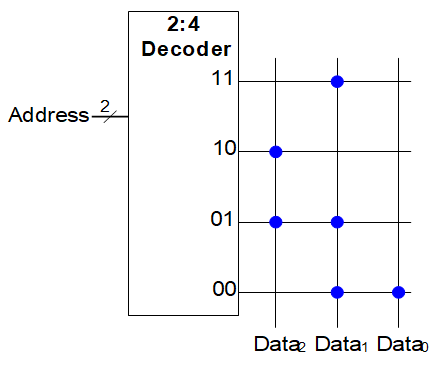
\includegraphics[width=\linewidth]{mem_logic.png}
        \label{fig:mem_logic}
    \end{figure}
    \end{minipage}
    \begin{minipage}[t]{0.49\textwidth}
    $$\text{Data}_0=\bar{\text{Addr}_1}\bar{\text{Addr}_0}$$
    $$\text{Data}_1=\bar{\text{Addr}_1}+\text{Addr}_0$$
    $$\text{Data}_2=\text{Addr}_1 \oplus \text{Addr}_0$$
\end{minipage}
\caption{Esempio logica}
\end{figure}

\subsection{Array logici}

Sono dei componenti in cui si svolgono operazioni logiche sequenziali.

\newpage

\paragraph{PLA}

\begin{itemize}
    \item M input
    \item zona AND
    \item N implicanti generati da quest'ultima
    \item zona OR
    \item P output
\end{itemize}

\begin{figure}[ht]
    \centering
    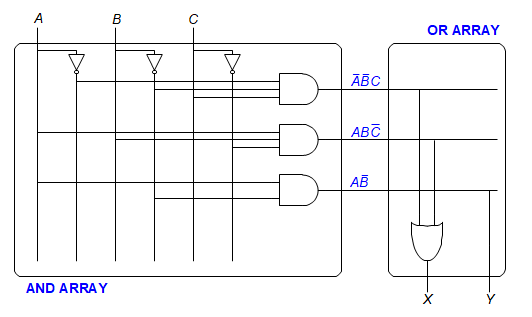
\includegraphics[width=\linewidth]{PLA.png}
    \caption{Esempio PLA}
    \label{fig:pla}
\end{figure}

\newpage

\paragraph{FPGA}

Composti da:
\begin{itemize}
    \item Elementi logici
    \item Elementi input/output
    \item Interconnessioni tra questi
    \item RAM e moltiplicatori (in alcuni casi)
\end{itemize}

\begin{figure}[ht]
    \centering
    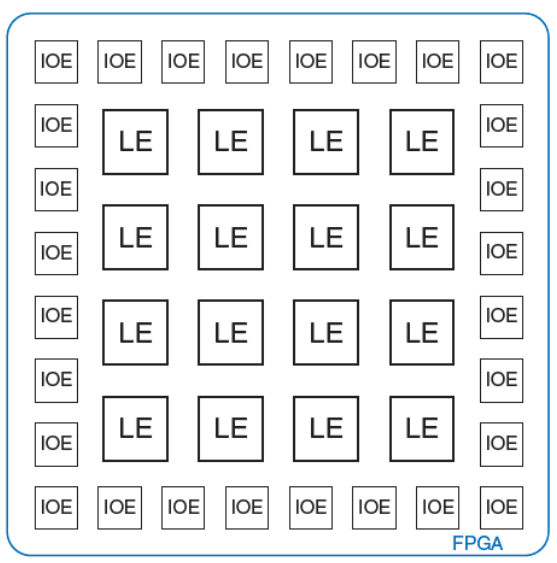
\includegraphics[width=.7\linewidth]{FPGA.png}
    \caption{Schema FPGA}
    \label{fig:fpga}
\end{figure}

Gli elementi logici sono composti a loro volta da:
\begin{itemize}
    \item Lookup tables
    \item Flip-flop
    \item Multiplexer
\end{itemize}

\newpage

\subsection{Altri blocchi}

\paragraph{Contatore}

Un contatore con $x$ output genererà in sequenza tutte le $2^x$ possibili combinazioni.

\vspace{3pt}

Se $x=3 \implies  (000,001,010,011,100,101,110,111,000,001,\ldots)$

\begin{figure}[ht]
    \centering
    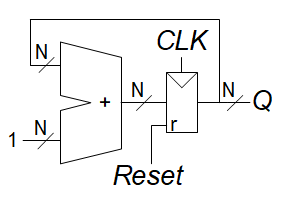
\includegraphics[width=0.5\linewidth]{counter.png}
    \caption{Schema contatore}
    \label{fig:counter}
\end{figure}

\paragraph{Shift register}

"Shifta" un nuovo bit In e l'ultimo bit Out ad ogni colpo di clock.

\begin{figure}[ht]
    \centering
    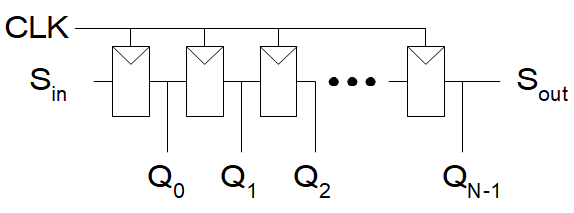
\includegraphics[width=0.7\linewidth]{shift_register.png}
    \caption{Schema Shift Register}
    \label{fig:shift_register}
\end{figure}

\section{Linguaggi descrittivi dell’Hardware
}

I linguaggi descrittivi dell’hardware servono a specificare funzioni logiche e produrne gli schemi ottimizzati.\newline

Permettono inoltre di simulare dei circuiti fornendo degli input e di generare una lista di tutti i componenti presenti e i loro collegamenti.

\subsection{SystemVerilog}

Si tratta di uno dei linguaggi di questo tipo più utilizzati.

\subsubsection{Sintassi ed altre cose basilari}
\begin{itemize}
    \item Case sensitive
    \item I nomi non possono iniziare con numeri
    \item Gli spazi sono ignorati
    \item Commento singolo //
    \item Commento  più righe /*  */
    \item Assegnamento bloccante con =
    \item Assegnamento non bloccante con $<$=
    \item Gli assegnamenti condizionali si possono fare con l'operatore ternario
    \item Sono presenti X e Z
    \item case() \ldots endcase è uno switch
    \item casez() contempla valori Z/?
    \item I numeri è opportuno scriverli nella forma $N'Bvalore$ con:
        \begin{itemize}
            \item N = numero di bit
            \item B = base usata (binaria,ottale,decimale,esadecimale),(b,o,d,h)
            \item valore = il numero
        \end{itemize}

    \item Si può inserire un delay tramite $\#x$ con x = numero di colpi di clock
        
\end{itemize}

\vspace{8pt}

Un modulo può essere descritto in 2 modi:
\begin{itemize}
    \item \textbf{Strutturale} = Descrivendo come i suoi sotto-moduli sono interconnessi
    \item \textbf{Comportamentale} = Descrivendo cosa deve fare
\end{itemize}

\subsubsection{Moduli comportamentali}

\begin{algorithm}[ht]
\caption{$Y=\bar{A}\bar{B}\bar{C}+A\bar{B}\bar{C}+A\bar{B}C$}
\begin{algorithmic}
\State module example(input logic a,b,c, output logic y);
   \State assign $y =\  \sim a\  \And\  \sim b \ \And \ \sim c\  | \ a\  \And \ \sim b\  \And\ \sim c \ |\  a\  \And \ \sim b\  \And \ c$;
\State endmodule
\end{algorithmic}
\end{algorithm}

\newpage

\subsubsection{Moduli strutturali}

\begin{algorithm}[ht]
\caption{NAND3}
\begin{algorithmic}
\State module and3(input logic a,b,c, output logic y);
   \State assign $y =a \And b \And c$;
\State endmodule
\State
\State module inv(input logic a, output logic);
   \State assign $y =\sim a$;
\State endmodule
\State
\State module nand3(input logic a,b,c, output logic y);
    \State // Definisco un segnale interno
   \State logic n1;
    \State
   \State // Definisco le istanze
   \State and3 andgate(a,b,c,n1);
   \State inv inverter(n1,y);
\State endmodule
\end{algorithmic}
\end{algorithm}

\vspace{-20pt}

\subsubsection{Array}

Si possono dichiarare array di bit tramite [i:j].\newline

Normalmente le operazioni tra array avvengono su tutti i bit se non meglio specificato, in alternativa si può ridurre un array ad una singola variabile (tramite operazione) facendo per esempio $y=\And a$.

\subsubsection{Logica sequenziale}

Si possono creare dei componenti singoli tramite il costrutto always @ (args), in particolare:
\begin{itemize}
    \item \textbf{always\_ff}: flip-flop
    \item \textbf{always\_latch}: latch
    \item \textbf{always\_comb}: logica combinatoria
\end{itemize}

\vspace{1pt}

\textbf{N.B. Bisogna rispettare la logica di funzionamento del componente scelto.}

\begin{algorithm}
\caption{D Flip-flop 2 bit}
\begin{algorithmic}
\State module flop(input logic clk,
                   input logic [1:0]d,
                   output logic [1:0]q);
   \State   always\_ff @ (posedge clk)
            \State \qquad \qquad q  $<$= d;
            
\State endmodule
\end{algorithmic}
\end{algorithm}

\end{document}
